%$$$$$$$$$$$$$$$$$$$$$$$$$$$$$$$$$$$$$$$$$$$$$$$$$$$$$$$$$$$$$$$$$$$$$$$$$$$$$$$$
% Paragraph : Linux Scalability : Fork intensive workload 문제점 설명 
%$$$$$$$$$$$$$$$$$$$$$$$$$$$$$$$$$$$$$$$$$$$$$$$$$$$$$$$$$$$$$$$$$$$$$$$$$$$$$$$$

\begin{figure}[h]
    \centering
    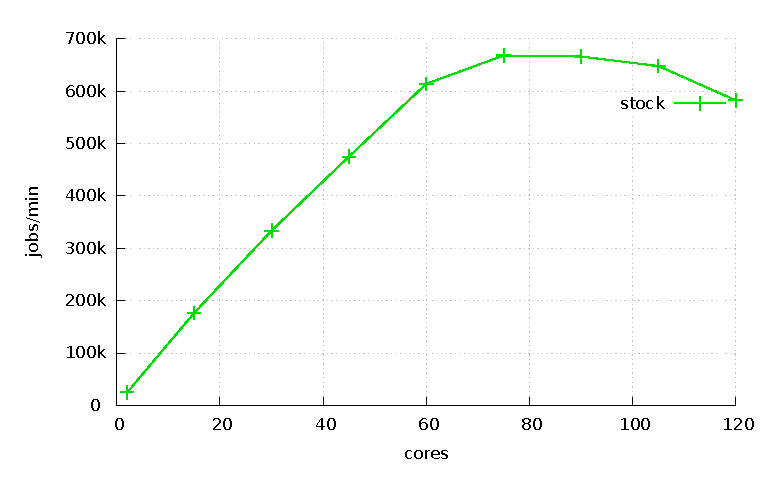
\includegraphics[width=0.8\textwidth]{graph/aim7_default}
    \caption{AIM7-multiuser 성능 확장성}
  \label{fig:aim7_default}
\end{figure}

\begin{figure}[h]
    \centering
    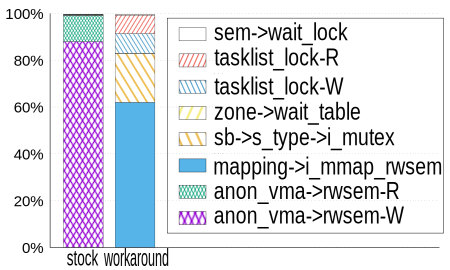
\includegraphics[width=0.8\textwidth]{graph/lockstat}
    \caption{120코어에서 락 때문에 기다리는 시간}
  \label{fig:aim7_default}
\end{figure}

운영체제 커널의 병렬화(Parallelism)는 시스템 전체의 병렬화에서 가장 중요한 부분이다.
만약에 커널이 확장성이 없으면, 그 위에 동작하는 응용프로그램들도 역시 확장성이
없게 된다~\cite{Clements15SCR}~\cite{Boyd-WickizerCorey}.
우리는 이처럼 중요한 운영체제 커널 중 멀티코어에 최적화된 리눅스 커널의 확장성을 분석하기 위해 
AIM7-multiuser 벤치마크를 사용하였다.
AIM7은 최근에도 성능 확장성을 위해 연구 진영과 리눅스 커널 커뮤니티 진영에서 활발히 사용되고 있는 
벤치마크 중 하나이다~\cite{Bueso2015STP}~\cite{Bueso2014MCS}.
AIM7-multiuser 워크로드는 동시에 많은 프로세스를 생성하며 디스크 파일(Disk File) 연산, 가상 
메모리(Virtual Memory) 연산, 파이프(Pipe), I/O(Input/Output) 그리고 수학 연산과 함께 수행한다.
우리는 파일 시스템의 성능 확장성을 최소화하기 위해, \code{tempfs}(Linux temp file system)를 사용하였다.
실험 결과 75코어까지 확장성을 가지나, 그 이후에서는 확장성이 떨어져 완만한 그래프를 보이는 문제점을 가진다. 

%$$$$$$$$$$$$$$$$$$$$$$$$$$$$$$$$$$$$$$$$$$$$$$$$$$$$$$$$$$$$$$$$$$$$$$$$$$$$$$$$
% Paragraph: Lockstat로 분석 결과 설명 
%$$$$$$$$$$$$$$$$$$$$$$$$$$$$$$$$$$$$$$$$$$$$$$$$$$$$$$$$$$$$$$$$$$$$$$$$$$$$$$$$
우리는 성능 확장성의 근본적인 문제를 분석하기 위해, 리눅스의
\code{lock\_stat}~\cite{LOCKSTAT}를 이용하여 120코어 부분에 락 경합을 분석하였다.
\code{lock\_stat}는 리눅스 커널에 있는 락 프로파일러(Profiler)이며, 
락을 얻기 위해 스레드가 얼마나 대기하였는지에 대한 대기 시간을 결과로 보여준다.
AIM7 벤치마크를 동작 시키고 120코어에서 락 경합을 분석 해보면, 
그림 ~\ref{fig:aim7_default}과 같은 결과를 얻는다.
실험 결과 AIM7 벤치마크는 익명(Anonymous) VMA(Virtual Memory Address)에서 상당히 많은 쓰기 락 경합이
발생한다.
이것은 수 많은 \code{fork}에 의해 프로세스를 생성하면서 발생하는 락 경합 문제이다.
리눅스가 \code{fork(), exit(), mmap()}시스템 콜(System Call)을 사용할 때 페이지(Page) 정보를
업데이트를 하게 되는데, 이 때 역 페이지 매핑(Revsers Page Mapping)의 연산이 이루어지고, 
동시에 락에 의해 스레드들은 직렬화가 된다. 

 \begin{figure}[h]
    \centering
    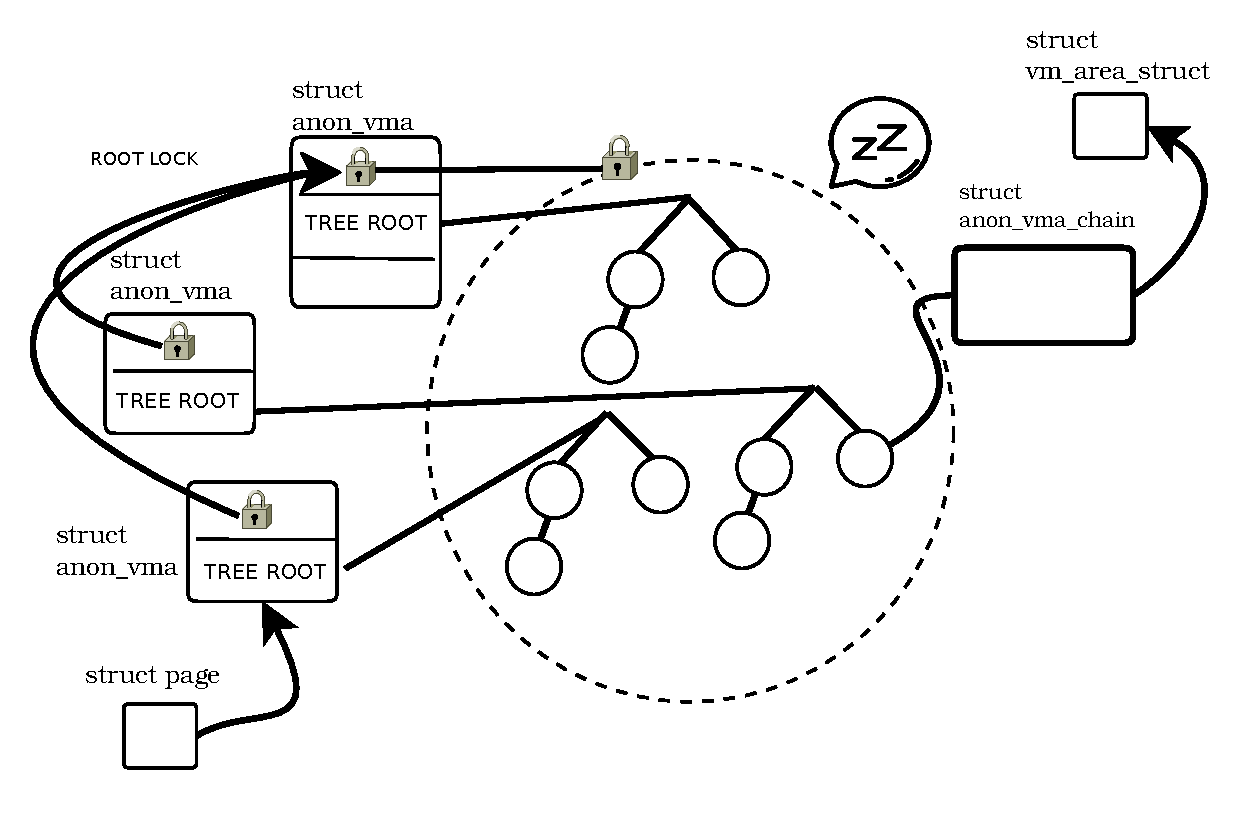
\includegraphics[width=0.8\textwidth]{fig/anon_vma_rmap}
    \caption{익명 역 매핑의 문제}
  \label{fig:anon_vma_rmap}
\end{figure}

다음으로 우리는 익명 역 매핑의 락 경합을 줄이기 위해, 임시로 \code{fork}에서 익명 역 매핑를 호출하는 부분과 
읽기 연산과 관련 있는 페이지 스왑(Page Swap)과 관련된 코드를 삭제하고, 다시 락 경합을 분석하였다. 
익명 역 매핑 관련 기능을 제거하면, 그 동안 상대적으로 가려졌던 파일 역 매핑에서 많은 락 경합이 발생되었다.
본 연구의 분석 결과 \code{fork}의 확장성 문제를 야기하는 것은 둘 중 하나가 아니라, 익명 역 매핑, 
파일 역 매핑 둘 모두 문제를 야기 한다고 볼 수 있다.

먼저 익명 역 매핑의 락 경합 문제는 그림~\ref{fig:anon_vma_rmap}이 보여준다.
그림은 물리적인 메모리 \code{struct page}에서 시작하여 그림의 오른쪽 상단의 
가상 메모리 영역인 \code{struct vm\_area\_struct}를 효율적으로 찾기 위한 과정을 보여준다. 
여기서 \code{struct anon\_vma\_chain}들은 모두 트리로 관리가 되며, 이 트리의 루트는
\code{struct anon\_vma}가 보관한다. 
모든 트리에 대한 연산은 \code{struct anon\_vma}가 가지고 있는 최상의 부모의 락에 의해 보호가 된다. 
따라서 \code{struct anon\_vma}의 모든 자식들은 모두 최상의 부모의 락 때문에 보호된다.
이것은 자식들의 트리 연산을 위해 접근하면 모두 블락에 걸리는 문제를 가진다. 
또한 파일 역 매핑의 락 경합 문제는 그림~\ref{fig:file_rmap_default}이 보이듯이 
익명 역 매핑 보다는 적지만, 트리에 접근하기 위해서는 \code{struct address\_space}의 락에 의해 
블락이 걸린다.

\begin{figure}[h]
    \centering
    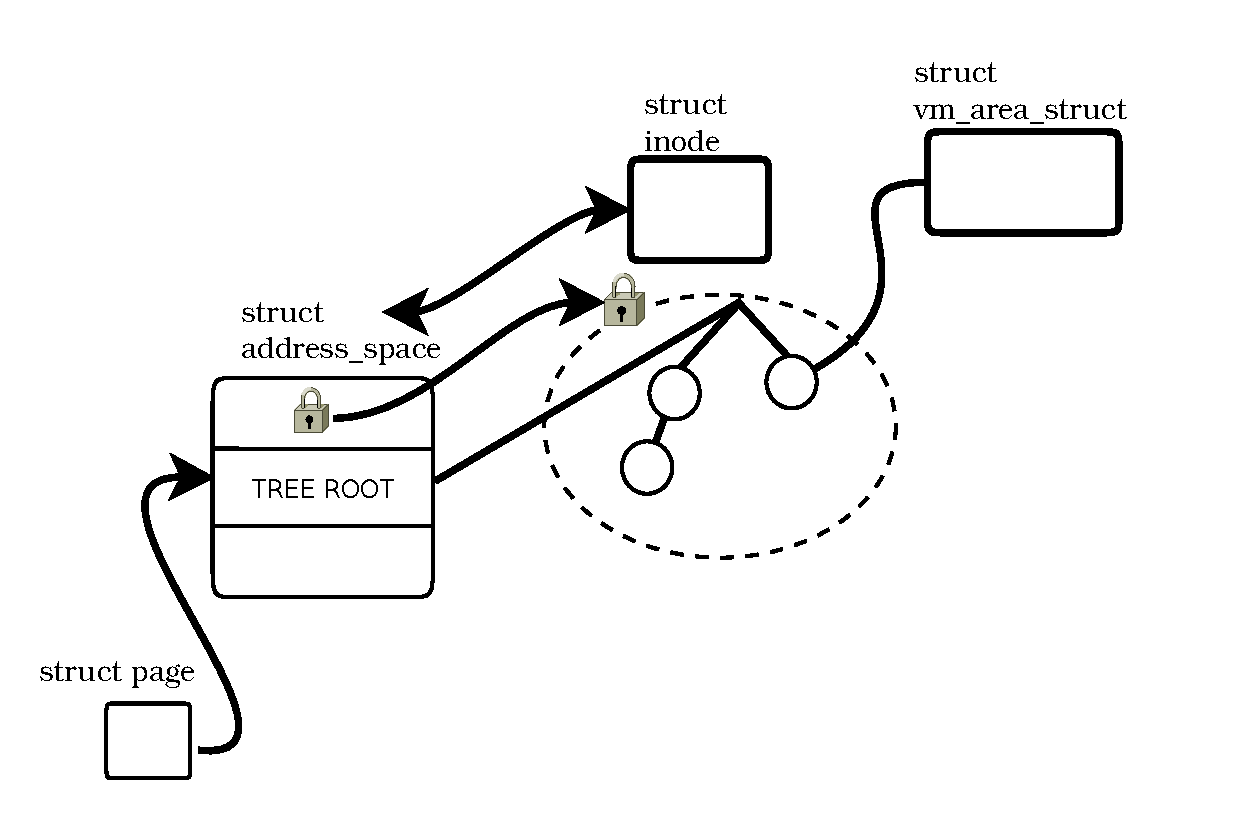
\includegraphics[width=0.8\textwidth]{fig/file_rmap_default}
    \caption{파일 역 매핑의 문제}
  \label{fig:file_rmap_default}
\end{figure}

%$$$$$$$$$$$$$$$$$$$$$$$$$$$$$$$$$$$$$$$$$$$$$$$$$$$$$$$$$$$$$$$$$$$$$$$$$$$$$$$$
% Paragraph : 리눅스 reverse page map의 write serialization 문제점
%$$$$$$$$$$$$$$$$$$$$$$$$$$$$$$$$$$$$$$$$$$$$$$$$$$$$$$$$$$$$$$$$$$$$$$$$$$$$$$$$
익명 역 페이지 매핑은 리눅스 커뮤니티에서 잘 알려진 락 경합 문제~\cite{Andi2011adding}이고, 
파일 페이지 역 매핑에 대한 락 경합 문제는 S. Boyd-Wickizer가 OpLog 논문을 통해 \code{fork}의 확장성 
문제의 중요한 원인으로 제시한 부분이다.
본 연구에서는 익명 역 매핑과 파일 역 매핑 두 가지 모두 개선해야지 \code{fork}의 성능 확장성이 
향상 된다는 것을 분석하였다. 

\begin{figure}[h]
    \centering
    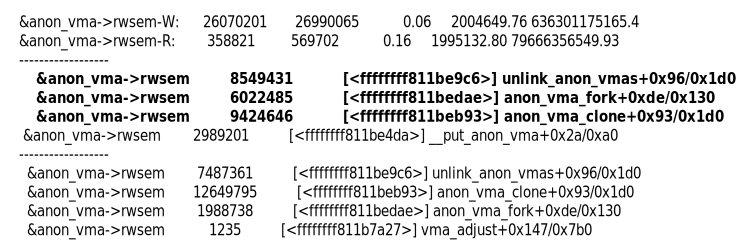
\includegraphics[width=0.8\textwidth]{fig/anon_vma_func}
    \caption{120코어에서의 lock\_stat 결과 분석}
  \label{fig:anon_vma_func}
\end{figure}

\begin{figure}[h]
    \centering
    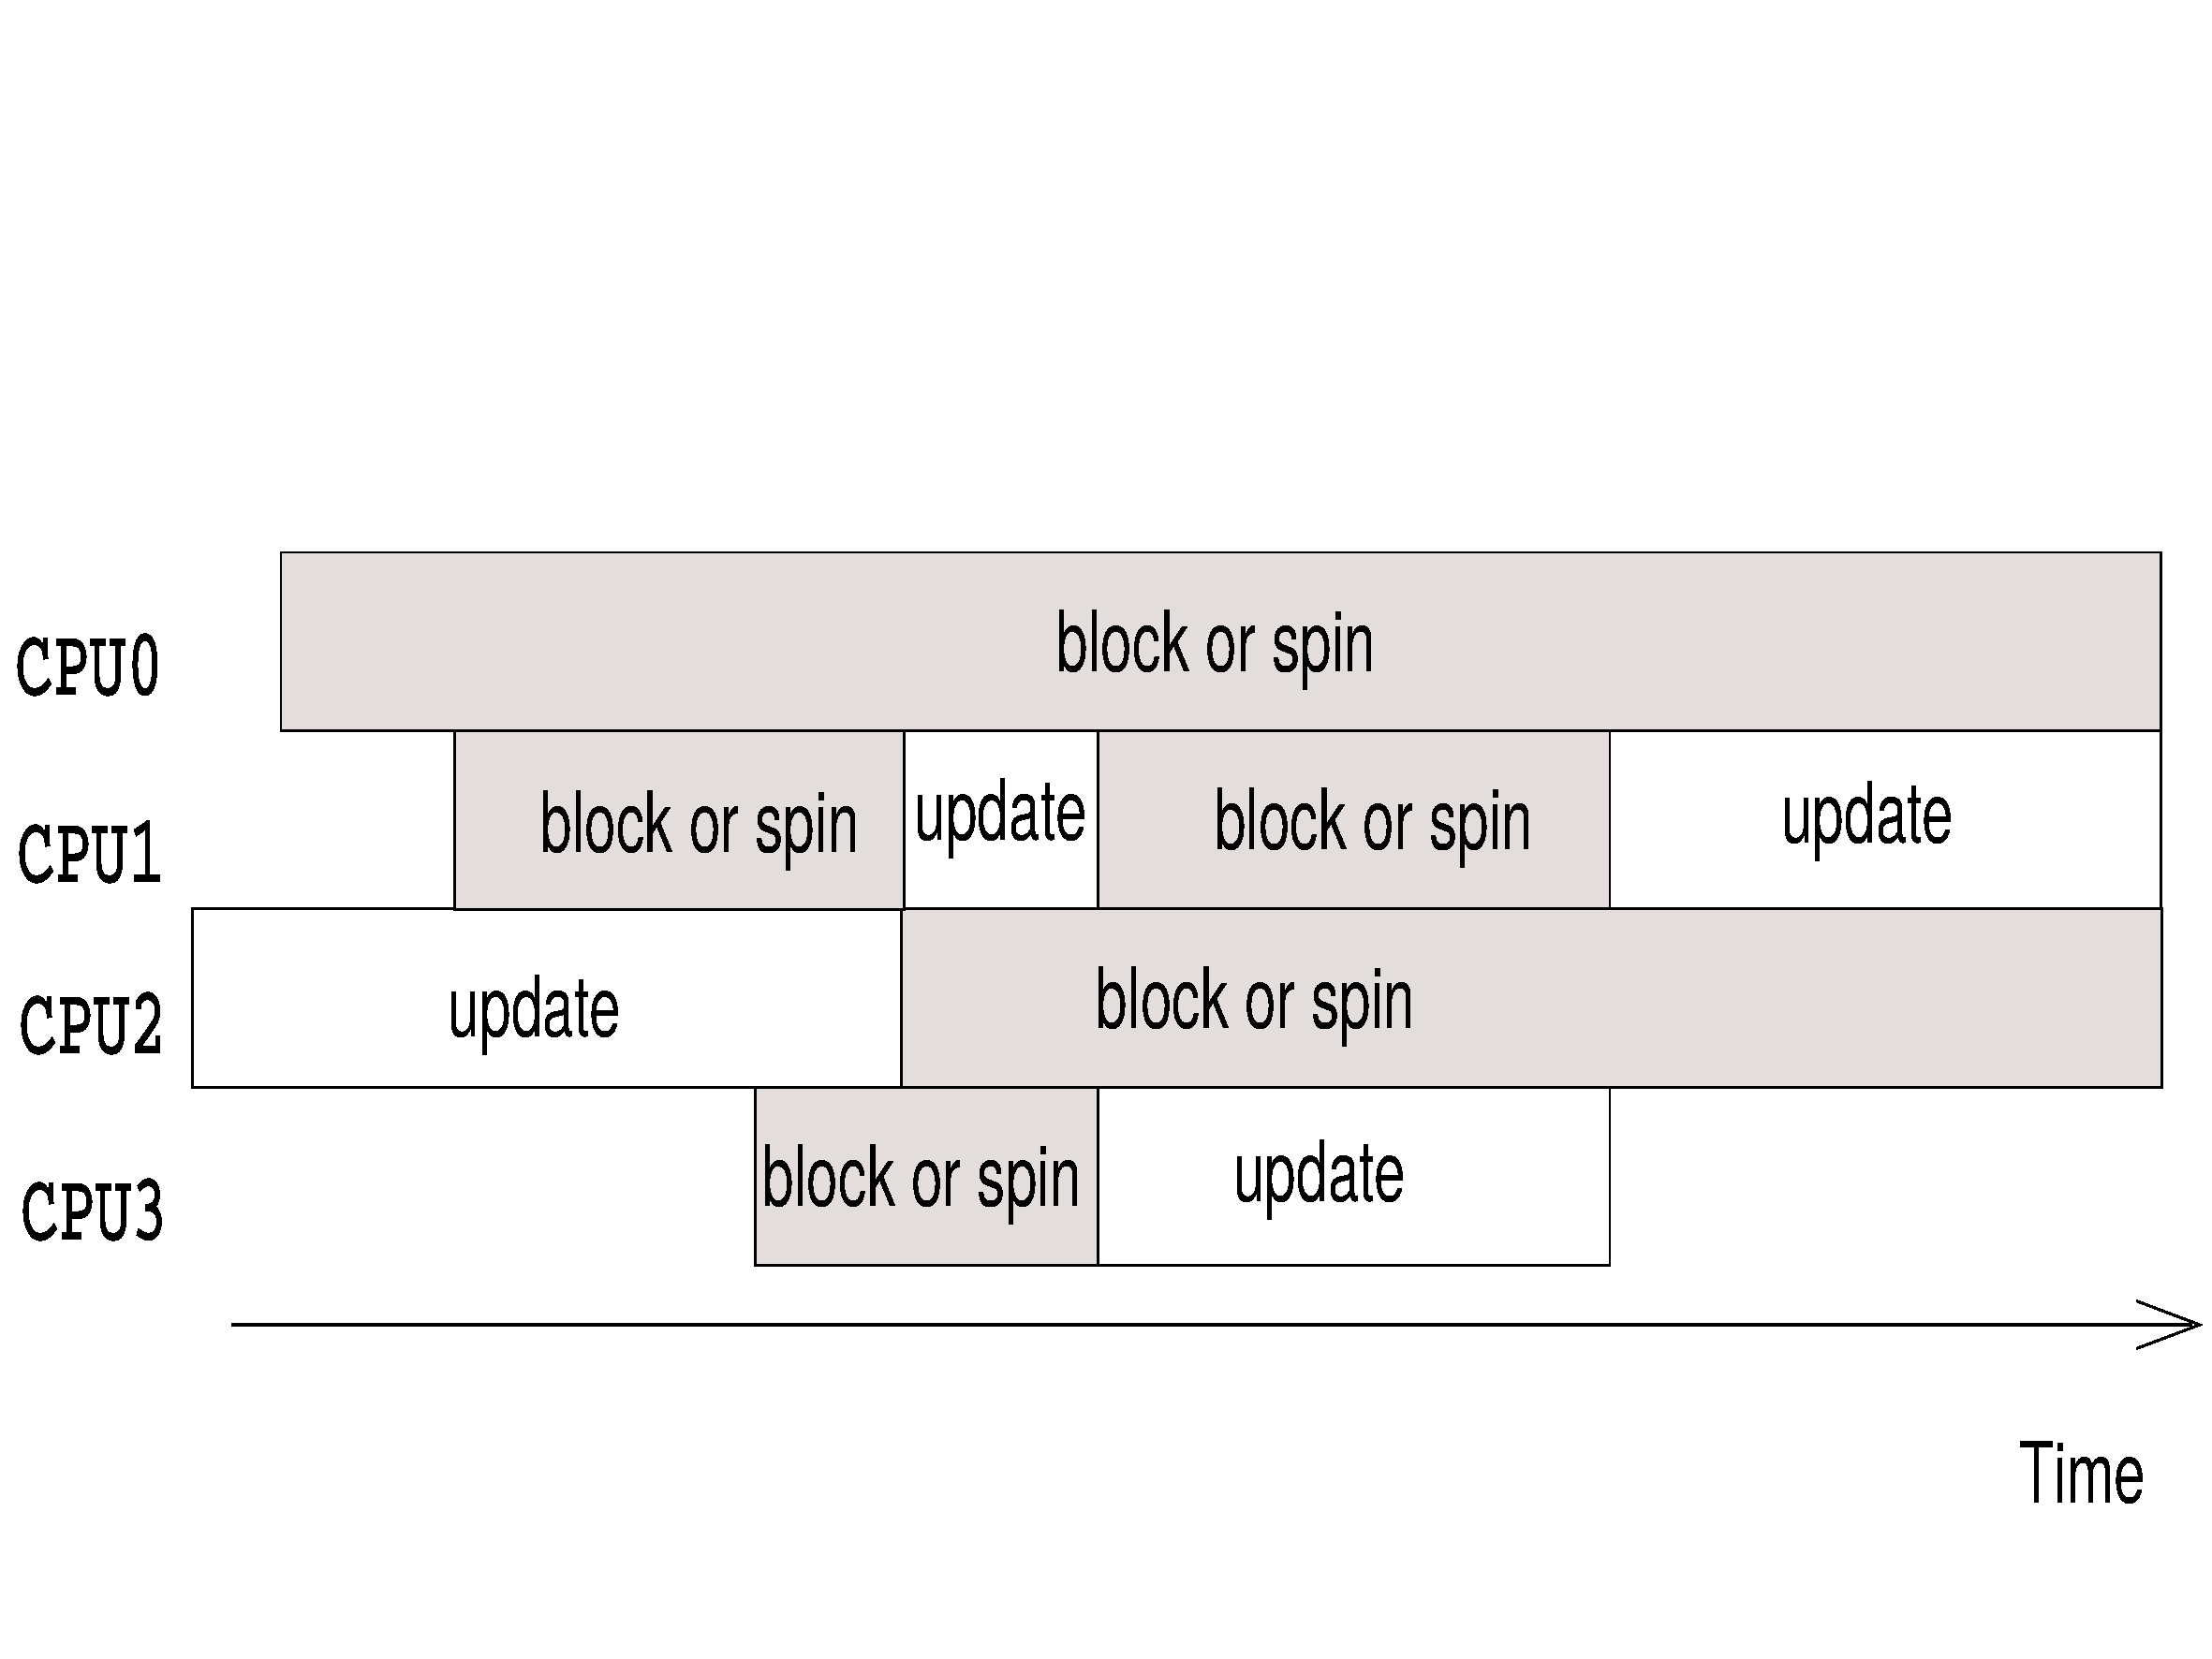
\includegraphics[width=0.8\textwidth]{fig/update}
    \caption{업데이트 직렬화의 문제}
    \label{fig:update}
\end{figure}

%$$$$$$$$$$$$$$$$$$$$$$$$$$$$$$$$$$$$$$$$$$$$$$$$$$$$$$$$$$$$$$$$$$$$$$$$$$$$$$$$
% Paragraph : update heavy한 상황에 대한 설명과 해결 방법에 대한 설명
%$$$$$$$$$$$$$$$$$$$$$$$$$$$$$$$$$$$$$$$$$$$$$$$$$$$$$$$$$$$$$$$$$$$$$$$$$$$$$$$$
락을 호출하는 함수들을 분석해보면 그림~\ref{fig:anon_vma_func}과 같다.
경합이 발생되는 함수(\code{unlink\_anon\_vma, anon\_vma\_fork, anon\_vma\_clone)}들의 
특징을 보면 대부분 자료구조 업데이트 연산을 수행하는 함수들이다. 
결국 높은 업데이트 비율이 때문에 락 경합이 많이 발생한 것이다.
업데이트 락 경합의 문제점은 그림~\ref{fig:update}와 같이 어떠한 동기화 기법을 사용해도 
결국 업데이트 연산에서는 직렬화가 된다는 것이다.

이처럼 높은 업데이트 비율 때문에 발생하는 업데이트 직렬화 문제를 해결하기 위해 그 동안 여러 방법이 
제안되었다. 
연구된 방법들은 논블락킹 알고리즘을 이용하는 
방식과 로그 기반 알고리즘을 사용하는 방법이 있다.
논블락킹 알고리즘들은 하드웨어 동기화 연산들을 활용하여
락과 같은 동기화 메커니즘 없이 업데이트와 읽기 연산을 수행하는 방법이다.
예를 들어, 논블락킹 알고리즘들은 업데이트 연산을 수행할 때, 업데이트를 원자적인 CAS(Compare And Swap) 
명령으로 전역 변수가 변경되었는지 확인한 후 수정하는 일을 수행한다.
만약 다른 스레드들에 의해 전역변수가 수정되었다면 CAS 연산은 실패되고, 업데이트 연산은 
처음 부터 다시 수행된다. 
결국 다른 스레드가 같은 메모리 주소의 내용을 변경을 안 할때까지 CAS를 이용해 반복 적으로 
확인하는 방법으로 동시적 업데이트를 보장한다. 
하지만 이러한 방법도 결국 공유 메모리 주소에 다수의 스레드가 CAS로 접근하여 병목 현상이 생긴다. 
이것은 결국 캐시 일관성 트래픽을 만든다~\cite{SilasBoydWickizerPth}.
최근에는 이처럼 캐시 일관성 트래픽 문제를 발생 시키는 연산을 줄인 로그 기반 방법들이 연구되고 있다.

%$$$$$$$$$$$$$$$$$$$$$$$$$$$$$$$$$$$$$$$$$$$$$$$$$$$$$$$$$$$$$$$$$$$$$$$$$$$$$$$$
%Paragraph : Log 기반의 알고리즘 대략적인 설명 
%$$$$$$$$$$$$$$$$$$$$$$$$$$$$$$$$$$$$$$$$$$$$$$$$$$$$$$$$$$$$$$$$$$$$$$$$$$$$$$$$
로그 기반 알고리즘은 업데이트 비율이 많은 자료구조에 적합한 알고리즘이다. 
로그 기반 알고리즘은 락을 피하기 위해 업데이트 연산이 발생하면, 자료구조의 업데이트 
연산(삽입 또는 삭제)을 함수 인자(Argument)와 함께 저장하고, 주기적 또는 읽기 연산이 
수행되기 전에 그 동안 저장된 로그를 수행하는 방법이다.
이러한 로그 기반 방법은 마치 CoW(Copy on Write)와 유사하다.
즉, 읽기 연산에 저장된 로그가 수행됨으로 읽기가 간헐적으로 수행되는 자료구조에 적합한 방법이다.

이처럼 업데이트 비율이 많은 자료구조를 위한 로그 기반 방법은 총 4가지의 장점을 가진다. 
첫째, 업데이트가 수행하는 시점 즉 로그를 저장하는 순간에는 락이 필요 없다. 
따라서 락 자체가 가지고 있는 캐시 일관성 오버헤드를 줄일 수 있다. 
둘째로, 저장된 순차적인 업데이트 명령을 하나의 코어에서 수행하기 때문에, 캐시 지역성이 높아진다.
셋째, 큰 수정 없이 기존 여러 자료구조(Tree, List)에 쉽게 적용할 수 있는 장점이 있다.
마지막으로 저장된 로그를 실제 수행하지 않고, 여러 가지 최적화 방법을 사용하여 적은 
명령으로 로그를 줄일 수 있다. 
LDU도 로그 기반 방법을 따른다. 그러므로 앞에서 설명한 로그 기반 방법의 장점을 모두 가짐과 동시에
업데이트 순간 삭제 가능한 로그를 지우는 최적화 방법으로 성능이 향상된다.

